There are several terms in the network domain, and this section will contain descriptions of networks and network theory, as well as definitions used in this report. 

The implementation of a communication network is necessary, as the sensor system is supposed to reduce the amount of work for measuring the soil status over the golf course. The current method of measurement is time-consuming, because of the travel time used to cover the designated area of the golf course. A network implementation of the sensor system can transmit the data gathered from each sensor to an end point where the data can be analyzed or processed.

A computer network is a collection of computers and devices connected so that they can share information and services \cite{mansfield2009computer}. Devices and connections in computer networks can be modeled with graphs, and therefore the network terminology used will be similar to graph terminology. Further on in this report, a device connected in a network will be called a node and the connection from one node to another will be called an edge.

%The communication structure the devices use to exchange information over a medium is called protocol, which will be described in another section.

%Definitions:
% Node: device in the network
% Edge: connection in the network
% Topology: arrangement/structure of objects
% Destination node: main node/gateway/ {[raspberry 3.14]}
% Gateway
% Relay
% Routing
% Flooding
% Data: transmitted information

A topology is any arrangement of objects that can be connected with edges \cite[p.~628]{discMath}. A network topology is the arrangement of the nodes, using edges as the structure. There are different types of network topologies and here are some examples:
\begin{itemize}
	\item Ring
	\item Line
	\item Bus
	\item Tree
	\item Star
	\item Mesh
\end{itemize}

A selection can be seen in figure \ref{fig:topologies}. The bus topology will not be considered, because it is not suited for a wireless network implementation \cite{re-find-it}. 
%The topologies considered for this use case are star, mesh, tree and ring networks. 

\begin{figure}[h!]
	\centering
	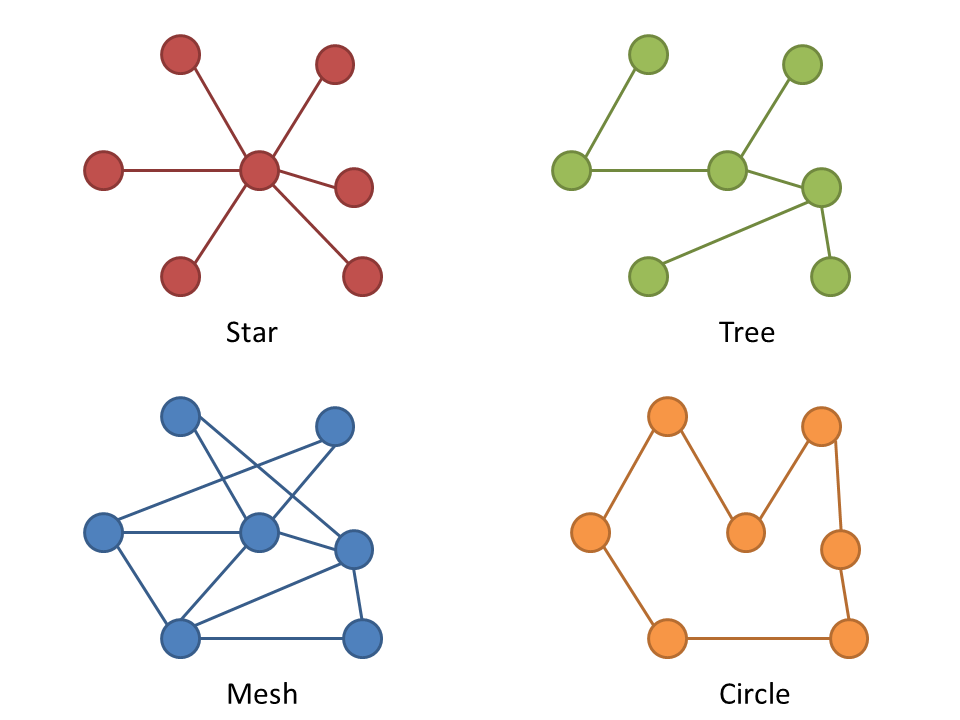
\includegraphics[width=0.8\textwidth]{figures/topologies.png}
	\caption{Network topologies.}
	\label{fig:topologies}
\end{figure}

The star topology, figure \ref{fig:topologies} a, has one main node that the other nodes are directly connected to. An example of a star topology network is wifi, typically with a wireless router to which other devices connect to gain network access. The wireless router will handle the network communication and redirect the information to the correct device. A limitation of the star network is that all nodes must have a direct connection to the main node, and therefore be clustered within the reach of the main node coverage. \todo{kilde}

A tree topology, figure \ref{fig:topologies} b, also utilizes a main node, called the root of the tree, but the devices in the network do not necessarily connect directly to the main node, but rather connect to another node that relays to the main node. This can repeat over multiple levels, so that information is relayed through several nodes, before reaching the main node. The tree network has a fixed node structure, and the relay nodes will route the information towards the destination. \todo{kilde} It has a reach advantage over the star topology, as data of nodes not directly within reach of the main node still can be received at the destination node.

The ring topology, figure \ref{fig:topologies} d, connects all nodes in a Hamilton circuit, where the path passes through all nodes exactly once. This topology does not require a central node to control the data communication, and will like the tree topology relay the data being sent through a certain chain of nodes before it reaches the destination node. It is vulnerable, while there is only two directions to communicate, and if a connection is lost, there could be a stop \todo{constipation?} in the data flow. If any one connection or edge is removed from the circuit, the remaining graph is a line, resulting in one chain of communication.

% It is a type of mobile ad hoc network.
Another topology is the mesh, figure \ref{fig:topologies} c. There are two kinds of mesh networks: The full-mesh and the partial-mesh networks. A full-mesh describes a network where all the nodes are interconnected, similar to a fully connected graph. In this topology, there will be no redirecting or relaying, but just a direct connection to the destination node, regardless which destination. A partial mesh is also a mesh network, but does not require all nodes to be connected, so that it's similar to a tree topology, but with cycles. The partial-mesh must then support relaying of data, to transfer data from any node to the destination node.

%The mesh networks have the same limitation as a tree network, regarding the information transmission delay because the information transmits through up to several nodes. \cite{g2wmn}

%The best fitting network topology for the use case is a mesh network. It can transmit information through the network without limiting the connected devices to a certain distance from a main device, as with a star topology. It is also capable of multiple methods of distributing information. It does not rely on all nodes working at all times, as the network can reconfigure and find another path of information. This applies as long as there somehow exists another node that can relay the information towards the main node.

\todo{Move this paragraph to protocols?}
There are multiple methods of communicating through a mesh network, therein routing and flooding are two alternatives. Routing will transfer the information to the destination node through a determined route, whereas the flooding method wil notify all nodes within reach to distribute the information forward, and this will repeat until all nodes has transmitted the information, and hence the destination node also has received the information.

%''\textit{An ad-hoc wireless network is a wireless network, comprised of mobile computing devices that use wireless transmission for communication, having no fixed infrastructure}'' - \cite{murthy2004ad}. 